\section{Convolution Neural Network}
\label{sec:cnn}
Perceptron algorithm has been proving their potential power by achieving many initial success. Most notable is the convolutional neural nets (convnets or CNNs), beginning with the model for handwritten digit recognition problems introduced by Yann LeCun at AT&T Bell Labs \cite{lecun1989backpropagation}. Nowadays, CNNs have become the essential technique in any module or state-of-the-art model of computer vision. In fact, the convolution operation tackles the exponential parameters growth by the weight sharing kernel.
% CNN as a feature extractor image here 

The first CNN architecture was introduced by Yan Le Cunn et al. \cite{lecun1989backpropagation} to process the visual data, which is inspired from the way human vison system works. One of the most common usage of the CNN is as a feature extraction module. It takes the images $H \times W \times C$ (or $H \times W \times D$) and extracts the information through multi-level downsampling layers, which is know as feature maps. Each smaller feature map holding the comprehensive information and relationship of nearby pixels. Feature map can also transform to another form, which is called feature vector.

\subsection{Convolution in signal-processing}
Convolution technique first appeared in the signal processing field. Given two signals $f$ and $g$ as two vectors with corresponding length are $m$ and $n$, $f$ is the input signal and $g$ is the kernel. The convolution definite output signal will be $h = f \ast g$. (equation \ref{eq:conv})
\begin{equation}
    \label{eq:conv}
    f \ast g(i) = \sum_{n=0}^{N-1}{g(n)f(i-n)}
\end{equation}
\begin{itemize}
    \item Stride is the number of element that the kernel skip as it slides on the vector. For example, when the stride is 2, the kernel moves 2 cell when it slides on the vector.
    \item Padding is the added cell to the original vector before applying the convolution operation. Without padding, the output of $1 \times 7$ with kernel $1 \times 3$ will be $1 \times 5$.
    The common padding technique using in signal processing is replicate the first and last value, which means to solve it with out shape changing. For example we will add the padding on the raw signal $f$ by assign $f(-1) = f(N-1) = 30, f(N) = f(0) = 10$ (figure \ref{fig:conv1d}).
\end{itemize}
\begin{figure}
    \centering
    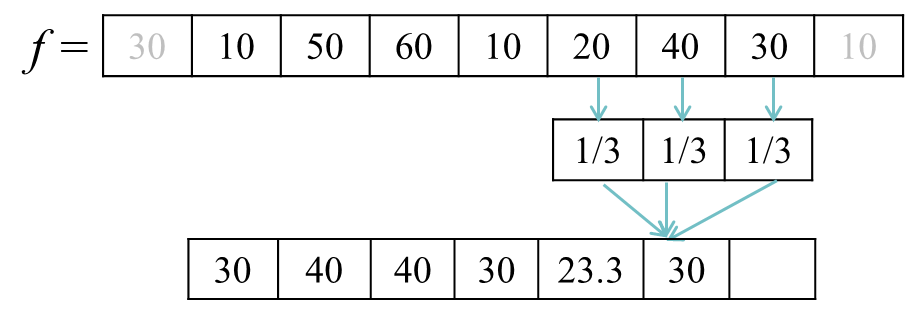
\includegraphics[height=1.2in]{content/resources/new_images/background/conv1d.png}
    \caption{Example of convolution 1D}
    \label{fig:conv1d}
\end{figure}

\subsection{Convolution in multi-dimension}
In image processing, convolution is an operator that combines the pixel information from neighbor pixels based on the kernel weight. The formal form of convolution operator in 2D is 
\begin{equation}
    f \ast g(x,y) = \sum_{m=0}^{M-1}{\sum_{n=0}^{N-1}{f(m,n)g(x-m,y-n)}}
\end{equation}
Where $f$ is the image size $M \times N$ and $g$ is the kernel. The intuitive illustration is show in fig \ref{fig:conv2d_op}. Visually, a convolution is imagined as sliding the filter across the image, and in each step it produce a value by taking the linear combination of nearby pixel.
\begin{figure}[h!]
    \centering
    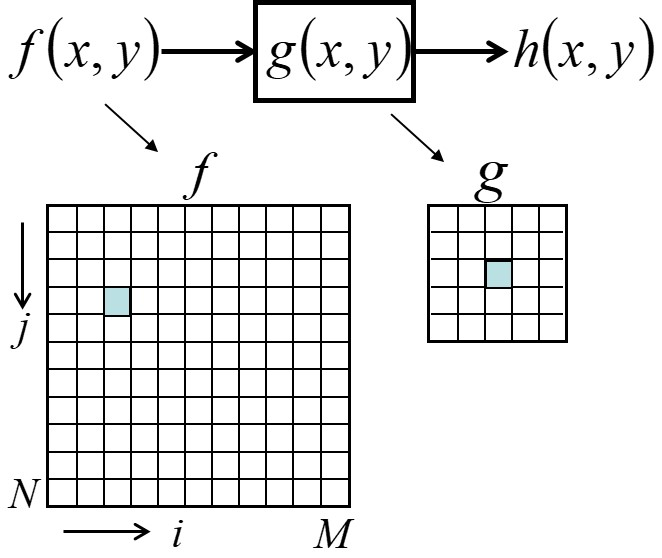
\includegraphics[height=2in]{content/resources/new_images/background/conv2d.jpeg}
    \caption{Illustration of convolution 2D}
    \label{fig:conv2d_op}
\end{figure}
As same as the convolution in one dimensional, convolution in image still faces some limitations. To deal with it, \textbf{stride} and \textbf{padding} have been used. The difference with one dimensional case is the kernel moves a number of stride value both vertical and horizontal when it slides; the common padding technique types are zero-padding and pixel-replicate-padding. However by extracting the information by convolution, the information loss occurs.
\begin{figure*}[t!]
    \centering
    \begin{subfigure}
        \centering
        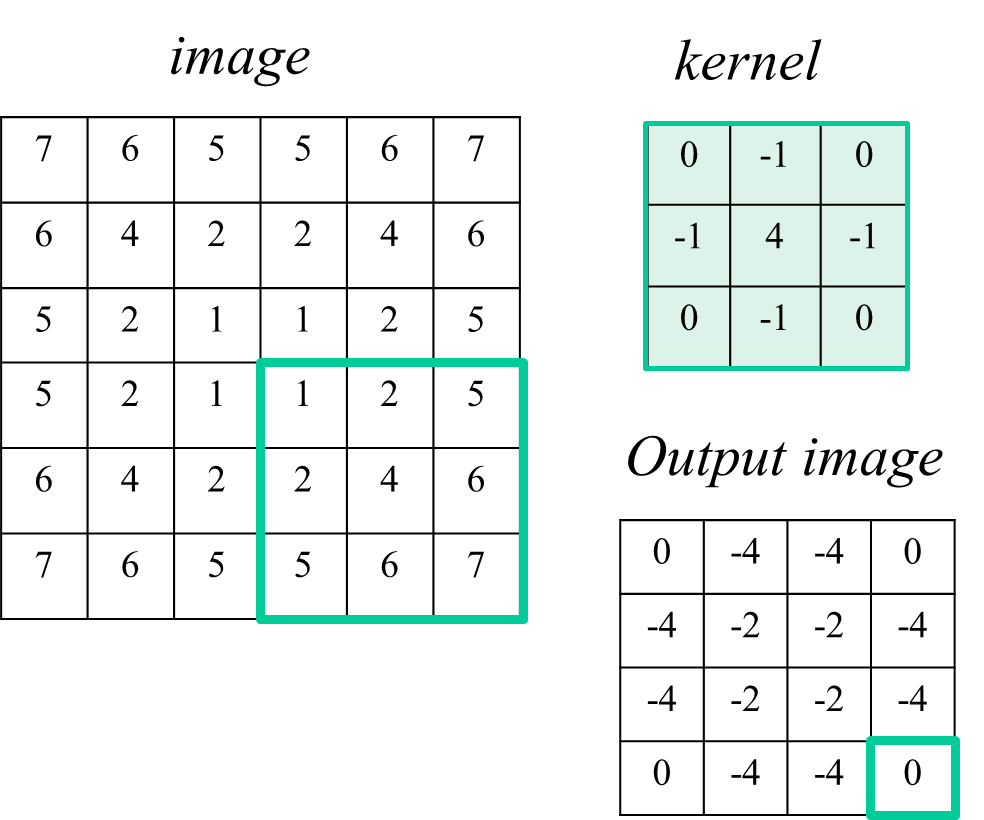
\includegraphics[height=2in]{content/resources/new_images/background/2dconv_nopad.png}
    \end{subfigure}%
    ~ 
    \begin{subfigure}
        \centering
        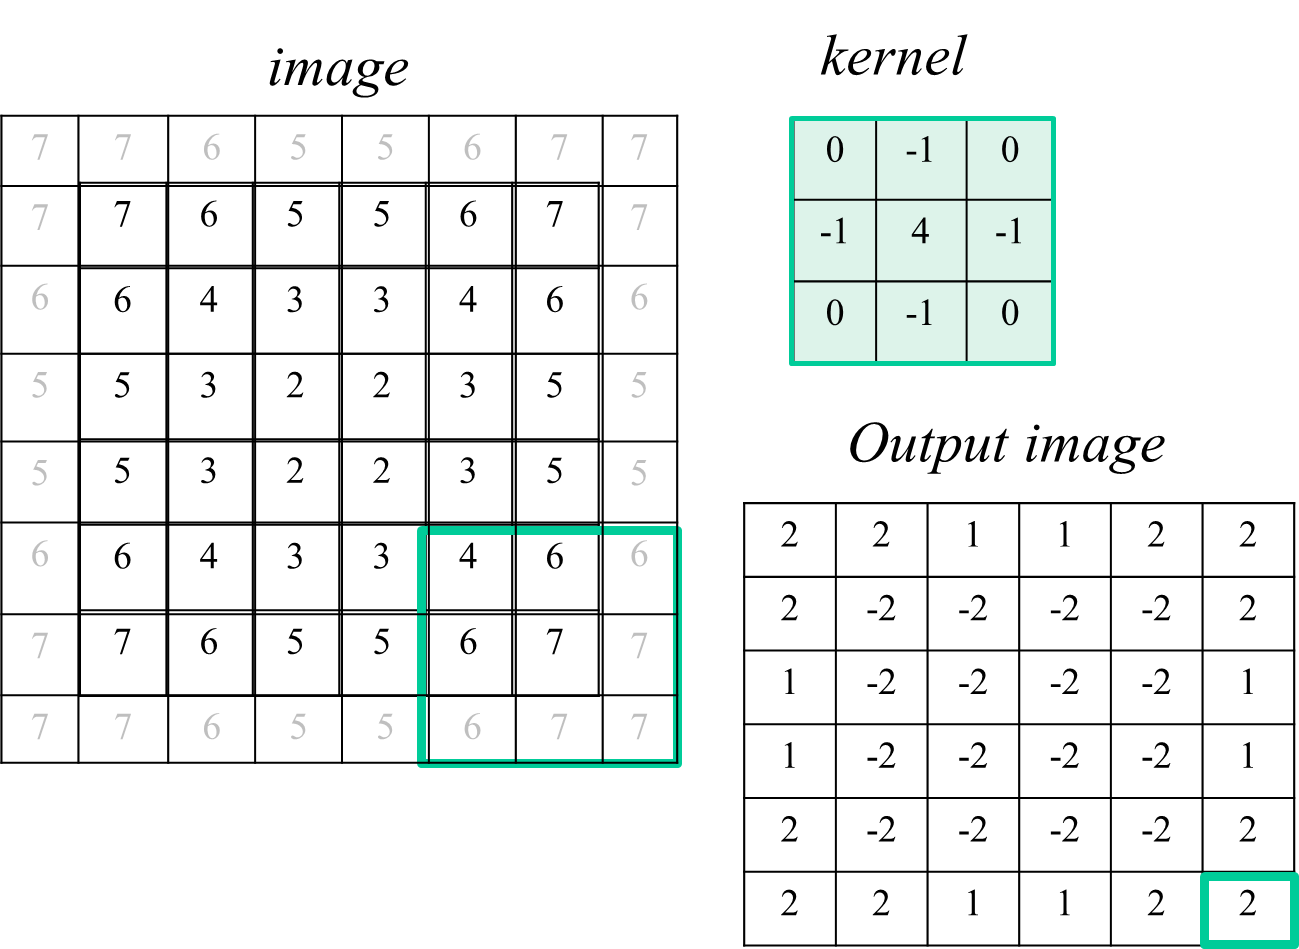
\includegraphics[height=2in]{content/resources/new_images/background/2dconv_padding.png}
    \end{subfigure}
    \caption{Comparation of convolution with padding (right) and without padding (left)}
\end{figure*}

The convolution operators appears long time ago, but inherits from the neural network strength, CNN is self generate the kernel parameters automatically. In other words, in the stage of training the network, the values of the kernel are “learned” from the given data by back propagation process. In addition to exploiting the spatial relationships, the kernel still holding less number of parameters than traditional feature extraction way.

\subsection{Pooling layer}
Pooling layer is use to reduce to image size. This lead to the efficiency in the reduction of the number of model parameters. The popular pooling types are max-pooling and average-pooling.
% \subsection{Popular convolutional neural network architecture}
% lenet + alex net
% vgg
% inception 
% resnet
% effnet 
% =))) 
